\documentclass[a4paper,12pt]{article}
\usepackage[utf8]{inputenc}
\usepackage[T1]{fontenc}
\usepackage{setspace} % This package is used to control linespacing; With \onehalfspacing for instance
\usepackage[danish]{babel}
\renewcommand{\danishhyphenmins}{22} % bedre orddeling
\usepackage{bm}
\usepackage{fnbreak}
\usepackage{sectsty}
\usepackage{wrapfig}
\usepackage[scriptsize]{caption}
\usepackage[danish,textsize=tiny,backgroundcolor=red,bordercolor=blue]{todonotes}
\usepackage[isbn,issn]{dk-bib}
\interfootnotelinepenalty=10000
\usepackage{graphicx}
\usepackage{usecases}
\usepackage{pdfpages}

\addto\captionsdanish{
\renewcommand\abstractname{Abstract}
}
%-----------------------------------------------------
\newcommand{\doctitle}{Assignment 1}
\newcommand{\docsubject}{02131 Embedded Systems}
\newcommand{\docauthor}{Cebrail, Jonathan og Christian}	
\newcommand{\docdate}{\today}
\newcommand{\docplace}{Danmarks Tekniske Universitet}
\newcommand{\HRule}{\rule{\linewidth}{0.5mm}}
%\newcommand{\docsubtitle}{Undertitle}
%-----------------------------------------------------

%-----------Scientific and mathematical packages begin-----------
% Math package
	\usepackage{amsmath}

% Vector symbols and functions (for example \vv)
	\usepackage{esvect}

% Mathematical symbols
	\usepackage{amssymb}
\DeclareMathOperator{\p}{\cdot}
\DeclareMathOperator{\N}{\mathbb{N}}
\DeclareMathOperator{\Z}{\mathbb{Z}}
\DeclareMathOperator{\C}{\mathbb{C}}
\DeclareMathOperator{\R}{\mathbb{R}}
\newcommand{\nn}{\nonumber}
% SI Units
	%\usepackage[output-decimal-marker={,}]{siunitx}		%http://mirrors.dotsrc.org/ctan/macros/latex/begincontrib/siunitx/siunitx.pdf
	%\sisetup{unitsep= \cdot }

% For Chemistry
	%\usepackage{chemscheme}		% http://ctan.org/pkg/chemscheme
	%\usepackage{chemsym}		% http://ctan.org/pkg/chemsym
	%\usepackage{mhchem}			% http://mirrors.dotsrc.org/ctan/macros/latex/contrib/chemstyle/chemstyle.pdf
	%\DeclareSIUnit\Molar{\textsc{m}}
%-----------Scientific and mathematical packages end--------------

% Non-default fonts - has to come _after_ some of the mathematical packages
\usepackage{pxfonts}

% Page margins
\usepackage[left=2.0cm, right=1.5cm]{geometry}

% Hyperref
\usepackage[colorlinks=true,linkcolor=black,citecolor=black,urlcolor=black]{hyperref}
%\usepackage[hidelinks]{hyperref}  
\hypersetup{pdftitle={\doctitle}} 
\hypersetup{pdfsubject={\docsubject}}
\hypersetup{pdfauthor={\docauthor}}

% Setspace
\usepackage{setspace}
\onehalfspacing
%\numberwithin{equation}{section}
% Alter some LaTeX defaults for better treatment of figures:
    % See p.105 of "TeX Unbound" for suggested values.
    % See pp. 199-200 of Lamport's "LaTeX" book for details.
    %   General parameters, for ALL pages:
    \renewcommand{\topfraction}{0.9}	% max fraction of floats at top
    \renewcommand{\bottomfraction}{0.8}	% max fraction of floats at bottom
    %   Parameters for TEXT pages (not float pages):
    \setcounter{topnumber}{2}
    \setcounter{bottomnumber}{2}
    \setcounter{totalnumber}{4}     % 2 may work better
    \setcounter{dbltopnumber}{2}    % for 2-column pages
    \renewcommand{\dbltopfraction}{0.9}	% fit big float above 2-col. text
    \renewcommand{\textfraction}{0.07}	% allow minimal text w. figs
    %   Parameters for FLOAT pages (not text pages):
    \renewcommand{\floatpagefraction}{0.7}	% require fuller float pages
	% N.B.: floatpagefraction MUST be less than topfraction !!
    \renewcommand{\dblfloatpagefraction}{0.7}	% require fuller float pages

	% remember to use [htp] or [htpb] for placement

% Title
\title{
\HRule \\
\textsc{\doctitle} \\
	 \small{\textsl{\docsubtitle}}
\HRule
}
\author{\docauthor\\\small{\docplace}}
\date{\docdate}

% Fancyheader : http://mirrors.dotsrc.org/ctan/macros/latex/contrib/fancyhdr/fancyhdr.pdf
\usepackage{fancyhdr}
\pagestyle{fancy}
\fancyhf{}
%\fancyhead[RO]{\docauthor \hfill \doctitle \hfill\thepage}
\fancyhead[RO]{\doctitle \hfill \docauthor \hfill \thepage /\ref{TotPages}}
% Get rid of annoying error messages
\setlength{\headheight}{14.5pt}
\usepackage{totpages}
\usepackage{sectsty}
\allsectionsfont{\scshape}
\begin{document}
\begin{titlepage}
\begin{center}
\textsc{\LARGE Danmarks Tekniske Universitet}\\[1.5cm]
\textsc{\large Embedded Systems 02131}\\[0.5cm]
\HRule \\[0.4cm]
{ \huge \bfseries Assignment 1}\\[0.1cm]
\HRule \\[1.5cm]
\end{center}
\begin{flushleft} \large
\emph{Gruppemedlemmer:}\\
Cebrail \textsc{Erdogan} s113414\\
Christian Mathias Rohde \textsc{Kiær} s123812\\
Jonathan Binner \textsc{Becktor} s123094\\
\end{flushleft}
\vfill 
\begin{center}
{\large \today}
\end{center}
\end{titlepage}
\newpage
\section*{Introduktion}
Vi har fået stillet til opgave at implementere Pan-Thompkins QRS detection algorithm. Algoritmens formål er at analysere et ECG signal og QRS komplekset. QRS komplekset giver det elektriske billede af ventriklernes sammentrækning. Et eksempel på et QRS kompleks ses på figur 1.\\
\begin{figure}[htp]
\centering
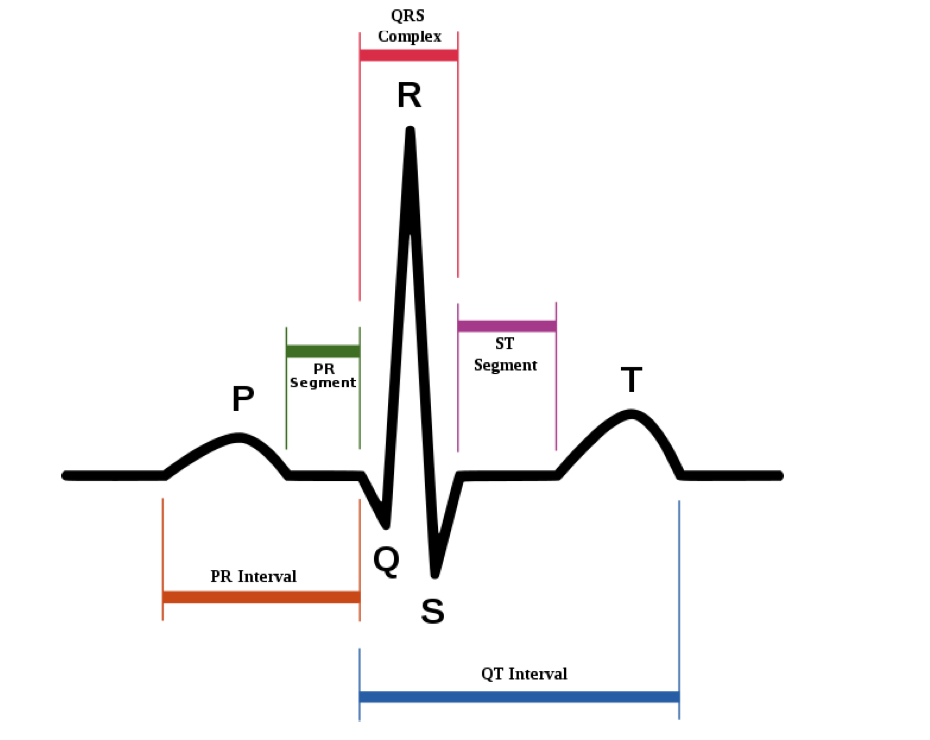
\includegraphics[scale=0.5]{qrs.png}
\caption{QRS Kompleks}
\label{Figur 1: QRS}
\end{figure}\\
Vores mål med algoritmen er derfor at give en vurdering af R peaks i QRS komplekset. Dette vil kunne alamere patienter om eventuelle hjerteproblemer. Vores algoritme skal derfor kunne registrere følgende:
\begin{itemize}
\item Intensiteten af R-peaks.
\item Varigheden af R-peaks.
\item Tiden siden sidste R-peak.
\item Advare hvis intensiteten af R-peaket er under en vis grænse eller hvis intervallet mellem R-peaks er ustabilt.
\end{itemize}
\newpage
\tableofcontents
\newpage
\section{Kravspecifikationer}
Vi vil her beskrive kravene for programmet, 
\subsection{Funktioner}
\subsubsection{Data erhvervelse}
Vores program skal kunne simulere en ECG måling. Der skal derfor indlæses et datasæt, som representere data fra en rigtigt patient, i realtime for så nøjagtigt som muligt at simulere en ECG måling.  
\subsubsection{Filtrering}
Da algoritmen kræver at datapunkterne behandles med stor præcision, anvendes 5 forskellige algoritmer til at filtrere den data vi har fået. De forskellige algoritmer gør alle noget forskelligt og meget spesefikt for datapunkterne. Low-Pass filtrer som i navnet lader de lave frekvenser komme forbi og blokerer de alt for høje. Highpass gør det modsatte. Derivative forstærker de signaler vi er interesseret i. Square filtrer tildeles for at vise større forskel mellem datapunkterne og for at gøre alle datapunkterne positive. Tilsidst bruges Moving window implementation filtret for at gøre signalet mere "blødt" altså at fjerne ekstra støj for at fobredre visualiseringen af R-peaks. De 5 filtre skal anvendes i følgende orden:
\begin{itemize}
\item Low-pass filter
\item High-pass filter
\item Derivative
\item Squaring
\item Moving window integration
\end{itemize}
\newpage
\subsection{Bruger output}
Programmet vil være i stand til at informere brugeren om praktiske oplysninger. I løbet af programmets kørsel vil brugeren blive informeret både om tekniske ting og advarsler angående patienten.
De tekniske data indeholder:
\begin{itemize}
\item Rpeak værdi: Værdien af nuværende Rpeak
\item RR interval: Tiden fra sidste Rpeak til nuværende
\item Pulse: Hjertets puls. Beregnet ved at sige:  ((250/RR\_ AVERAGE1)*60).
\end{itemize}
Alarmering:
\begin{itemize}
\item Rpeak under 2000: Skyldes for svag hjerteslag.
\item RR intervallet er ikke mellem RR\_ LOW og RR\_ HIGH 5 gange i træk: Skyldes usædvanlig interval mellem hjerteslag.
\end{itemize}	
\begin{figure}[htp]
\centering
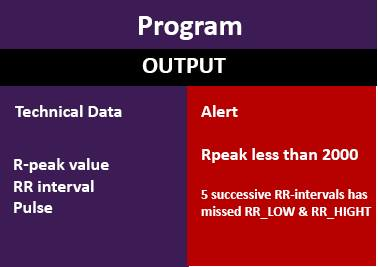
\includegraphics[scale=0.7]{output.jpg}
\caption{Output til brugeren}
\label{what up}
\end{figure}
\section{Programdesign}
\subsection*{Struktur}
Vi har taget udgangspunkt i de udleverede program filer til senoren, og efterfølgende oprettet klasser for alle filtre og QRS-registrings delene af programmet. Vi har en main klasse der kører selve programmet, og derfra kalder de nødvændige funktioner.\\
Filtrene er oprettet med navn, og funktionerne i det pågældende filter bliver derfra kaldt (eks. er low-pass filteret oprettet som lowPass.c). R-peak registrering forgår i QRS.c, hvorfra også udregningerne af intensiteten, varigheden og tiden siden sidste R-peak foregår.\\
Opdelingen er sket på denne måde, da vi synes en klasse for hver filter gav mest overskuelighed. Det er meget let derfra at gå ind og rette på en enkelt del af et givent filter, uden det giver problemer i resten af programmet. At holde QRS funktionerne adskildt fra resten af programmet giver samme fordele. Nedenfor ses et klassediagram for vores program.
\begin{figure}[htpb]
\centering
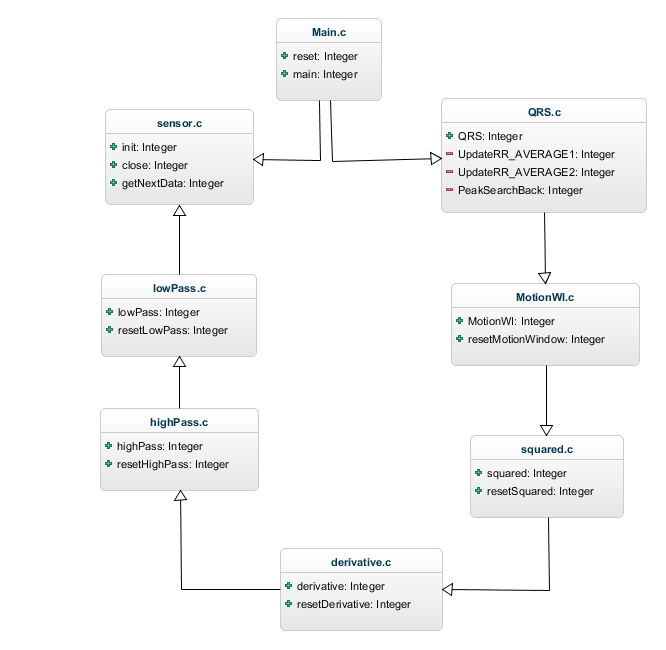
\includegraphics[scale=0.4]{fisse.jpg}
\caption{Klassediagram}
\label{Figur 2. Klassediagram}
\end{figure}
\newpage
\subsection{Data indlæsning}
Da programmet skal forestille at være en simulation af en ECG måling, ved brug af Pan-Thompsons QRS detection algorithm, skal programmet kunne læse data fra en fil. Til dette har vi vidreudviklet på sensor.c filen, og implenteret funktionen getNextData(). Dette vil give os muligheden for at hente data fra en fil, og bruge dette datasæt til analyse af QRS detection algoritmen. Sensor.c bruges derefter i main.c og henter alle vores signal data ind til analysen.
\section{Implementering}
\subsection{Filtre}
De forskellige filtre er belvet implementeret i hver sin klasse. Her er en gennemngang af nogle af dem da nogle af dem er meget ens hvor det eneste der gør dem forskellige er den matematiske formel.

\subsubsection{Low-Pass, High-pass, Derivative og Moving window implementation}
Her initializeres 2 arrays en til resultaterne og en til dataen. Størrelsen af arrayet afhænger af hvor langt tilbage formlen siger vi skal have resultater fra. Fx. skal vi have $x_{n-12}$ i Low-Pass filtret, vi skal altså have et array der gemmer x værdierne til og med $x_{n-12}$. Det bliver gjort med en forløkke som sætter den positon næste lig den forrige.
Hvorefter vi så returner resultatet. Derudover har vi også tilføjet en reset metode hvis man skal bruge filtrene igen. Den sætter bare alle positionerne i arraysne til nul.

\subsubsection{Squared}
Squared filtret ligger også i sin egen klasse. her får den input fra Derivative og returner inputtet ganget sig selv.

\subsection{QRS Detection algorithm}


QRS algoritmen er uden tvivl den vigtigste komponent i hele systemet. Den har til formål at finde ”peaks” – altså toppe – og behandle de fundne peaks. Algoritmen gør det muligt at fortolke frekvenserne. Nogle af de fundne peaks vil blive fortolket som hjertepuls (Rpeaks), mens nogle af dem fortolkes som støj. Hvis intervallet mellem Rpeaks er usædvanligt vil programmet kommet med output - advarelser. De essentielle dele af algoritmen bliver uddybet nedenfor.
\subsubsection{peaks}
Peaks er simple at finde. Der hentes data fra filteret. De hentes en ad gangen, men man kunne også hente tre ad gangen. Grunden til at der skal bruges tre ”datapoint” skyldes betingelsen:
$Xn-1 < xn, xn > xn+1$  ,  
\subsubsection{Gemme peaks}
Peaks er defineret som ”struct”. Struct gør det muligt at oprette et object og give den forskellige variabler. Så alle vores peaks har variablerne ”value”,”RR” og ”index”.
Nu er peak en type som kan tildeles. De fundne peaks gemmes i et array med typen peak. 

\subsubsection{Beregning af RR intervallet}

Intervallet af Rpeaks afgøre patientens tilstand, derfor er det også dem der bruges til at de forskellige udsagn i algoritmen. Vi beregner intervallet ved at sige:
Datapoint\_index  - index of last $Rpeak = interval$
Hvis RR intervallet ligger mellem RR\_LOW og RR\_HEIGHT er der intet galt, men hvis dette viser sig ikke at være tilfældet i 5 gange i træk, vil programmet komme med en advarsel. De seneste RR intervaller gemmes i en array med størrelsen 8, de fundne bruges til at finde gennemsnittet.

\subsubsection{Søg baglæns for peaks}
Når intervallet ikke er mellem RR\_LOW og RR\_HEIGHT vil den blive tjekket om den er større end RR\_MISS, hvis det er tilfældet vil den starte proceduren ”searchback”. 
I ”searchback” gennemsøger vi baglæns gennem alle de fundne ”peaks” indtil videre.
Lige så snart vi har en peak som er større end THRESHOLD2 fortsætter vi til algoritmens sidste step. Hver gang der betingelsen ikke er opfyldt går vi en skridt tilbage i arrayet.
 


\newpage
\section{Resultater}
Resultaterne er som ventet når "patienten" har problemer med hjertet får vi en advarsel og vi finder alle andre Rpeaks.\\
Vi har derudover lavet en performance analyse af algoritmeten. Vores test PC har været en maskine med en i7 2.2ghz quadcore processor med 45 watt strømforbrug. Maskinen kørte programmet med den store ECG10800K.txt fil. Programmet kørte med ca. 25\% af maskinens CPU kraft under udførslen. Performance chartet for kørslen af programmet kan ses nedenunder:
\begin{figure}[htp]
\centering
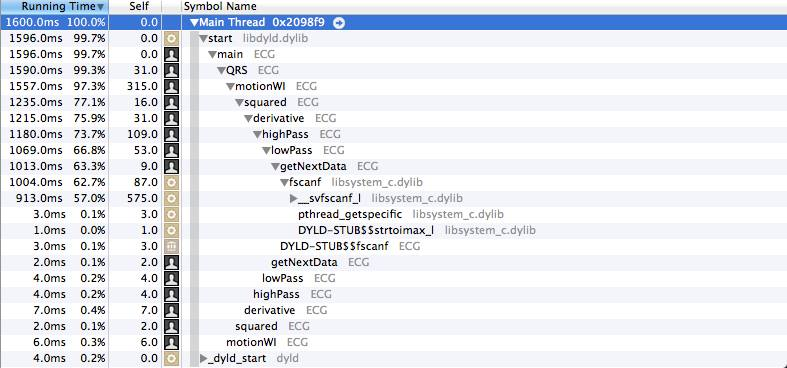
\includegraphics[scale=0.6]{CPUperformance.jpg}
\caption{CPU performance chart ved brug af ECG10800K.txt}
\label{CPU performance chart ved brug af ECG10800K.txt}
\end{figure}\\
Det vides at bærbare ECG skanner skal kunne læse 250 punkter i sekundet. Ud fra dette kan det udregnes hvor stort watt forbrug en bærbar maskine vil have, ved brug af QRS algoritmen. Vi udregner først hvor mange clockcycles processoren bruger ved kørsel på en kerne i 1.60 sekunder:
\begin{align*}
clockscycles\_overall = 2.2 \cdot 10^9 hz \cdot 1.60s	 = 3.52 \cdot 10^9 clockcycles
\end{align*}
Vi regner derefter ud hvor mange clockcycles der kører for hver linje:
\begin{align*}
clocks\_per\_line = \frac{3.52 \cdot 10^9}{10800000 } = 325.93 \frac{clocks}{line}
\end{align*}
Vi kan derefter regne ud hvor mange watt der bruges per linje på vores test pc. Da maskinen var på 25\% og har et strømforbrug på 45w, er strømforbruget under kørsel af programmet på 11.25w.
\begin{align*}
joules\_per\_line = \frac{325.93 \frac{clocks}{line}}{2.2 \cdot 10^9hz} = 0.00000167 \frac{j}{line}
\end{align*}
Da det vides at den bærbare enhed skal kunne læse 250 linjer i sekundet, kan det udregnes hvad strømforbruget vil være.
\begin{align*}
watt = 0.00000167\frac{j}{line} \cdot 250 = 0.00042w = 420 microwatt
\end{align*}
Dette gør algoritmen meget effetktiv i en bærbar enhed, pga den gode hastighed og det lave strømfobrug. Derudover kræves der ikke meget af hardwaren for at benytte algoritmen.\\
Koden optog ca. 2.5 mb RAM mens det kørte, hvilket også stiller et forholdsvis lavt krav til hardware specifikationer. 
\newpage
\section{Diskussion}
Vi som gruppe havde alle lavet en forskellig version af programmet og så senere merget det og fået et program som virker som det skal. Vi var i tvivl hvordan vi skulle håndtere alle de forskellige variabler der ville komme og havde rigtigt mange store arrays sat op, vi fant dog ud af at bruge structs for at have noget der minder objekter.\\\\
Hvis vi skulle finde en hardware løsning til dette kan vi se på figur 3 og se hvilke dele af programmet som kører langsommest så vi kan finde ud af hvor lidt hardware vi egentlig har brug for.Det er tydeligt i køretiderne fra processoren
at det der bruger længst tid er indlæsningen af data. Da det er en enhed som modtager maks ca. 220 datapunkter i minuttet kan vi se bort fra det. Da programmet ikke behøver at være meget hurtigt kan vi fokusere på at gøre det så energi besparende som overhovdedet muligt. Vi kan se at det som bruger nest mest energi er motionWI metoden som er en af filtrene der bruges til at gøre datapointse mere overskuelige. Den og alle de andre filtre kunne jo eventuelt hardcodes som hardware så der skulle bruges så lidt processor kraft som overhovdet muligt men igen størrelsen er jo altafgørende.
\newpage
\section{Konklusion}
Der gives et overblik over hvordan et kompliceret software bygges og hvilken undersøgelser den skal igennem for at blive betragtet som ”god software”.  Programmet blev bygget i tre faser. Første fase omhandler filtre , anden fase omhandler QRS og som sidste fase analysere vi programmet. Programmet simulere en ECG pulsmåler ved at hente data fra txt-filer. \\

Filtrene består af fem komponenter som har hver deres formål, at implementere dem var simpelt, da de alle sammen består af enkelte formler. \\

QRS algoritmen var derimod meget udfordrende.  De enkelte trin i algoritmen kræver omhyggelig implementering. Det er let at lave fejl når man har med en så stor algoritme at gøre. \\

Analysering af programmet viste, at den ville fungere meget godt som bærbart enhed. Der blev hverken brugt meget CPU eller hukommelse, derfor er programmet godt optimeret. \\

Programmet giver en god eksempel på hvordan software implementeres i den 
virkelig verden, fordi man også tænker på hardwaredelen i baghovedet. \\

De kommende opgaver kommer til at handle om hardware-simulation, hvilket vil give os forståelse for hardwaredelen. \\
\newpage
\section{Bilag}
\subsection{HelloWorld.c}
\begin{verbatim}
#include <stdio.h>

int main(int argc, const char * argv[])
{
    printf("Hello, World!\n");
    return 0;
}
\end{verbatim}
\subsection{ReadFile.c}
\begin{verbatim}
#include <stdio.h>

int main(int argc, const char * argv[])
{
    static const char filename[] = "/users/christiankiaer/Downloads/ECG.txt";
    FILE *file = fopen ( filename, "r" );
    
    int maxReading;
    int i1;
    while (fscanf(file,"%i",&i1) != EOF)
    {
        if (i1 > maxReading)
        {
            maxReading = i1;
        }
    }
    
    printf("The highest EKG reading is: %i", maxReading);
    return 0;
}
\end{verbatim}
\end{document}